\documentclass[a4paper,11pt]{article}

\usepackage{exptech}
\usepackage[colorlinks=true, linkcolor=black]{hyperref}

%Décommanter pour la relecture (interlignes plus importantes)
%\linespread{1,6}

%%%%%%%%%%%%%%%%%%%%%%%%%%%%%%%%%%%%%%%%%%%%%%%%%%%%%%%%%%%%%%%%%%%%%%%%%%%%%%%

\title{ \textbf{Création d'un modèle 3D à partir de dessins 2D} }
% Pour avoir le titre de l'expose sur chaque page

\author{ Aurélien \textsc{FONTAINE} Etienne \textsc{GEANTET} \\
	Manutea \textsc{HUANG} Arnaud \textsc{MARTIN} \\
	\\
	Encadrants : François \textsc{LEHERICEY}	Bertrand \textsc{COUASNON}}

\date{4 Mai 2015}                    % Ne pas modifier

%%%%%%%%%%%%%%%%%%%%%%%%%%%%%%%%%%%%%%%%%%%%%%%%%%%%%%%%%%%%%%%%%%%%%%%%%%%%%%%

\begin{document}

\maketitle                 % Génère le titre
\thispagestyle{empty}      % Supprime le numéro de page sur la 1re page

\begin{abstract}
	Lors de leur troisième année, les étudiants de l'INSA de Rennes doivent réaliser un projet. Notre groupe a choisi de travailler sur le développement d'une application sur tablette. Cette application est destinée à être utilisée lors de séances de démonstration dans la salle de réalité augmentée Immersia. Nous devons permettre au sujet de la démonstration de réaliser simplement et sans besoin d'explications sur le fonctionnement de l'application, des objets 3D à partir de dessins 2D qu'il aura fait. Une fois sa création effectuée, elle doit être envoyée vers la machine gérant la salle.
\end{abstract}
	
	\section{Introduction}
		%Présentation succinte du projet
		Au cours de ce rapport, vous trouverez les choix faits pour développer cette application. Tout d'abord, la sélection des technologies les plus à même de respecter le cahier des charges. Ensuite comment à partir de ces choix, nous avons défini l'architecture de l'application. Sur chaque partie de celle-ci, vous verrez les choix réalisés par l'équipe. Puis nous présenterons notre répartition du travail et le suivit de celui-ci au sein de notre équipe. Pour finir, nous concluons sur les objectifs atteints et les futurs possibles pour le développement de cette application.
	\section{Cahier des charges}
		Notre client nous a imposé le cahier des charges qui suit:
		
		-Supportable par Android Tablette
		-Application ergonomique: utilisation rapide pour un nouvelle utilisateur
		-Outils de dessin
		-Création d'objet 3D depuis les dessins ainsi fait
		-pouvoir exporter la création vers un serveur Unity
	\section{État de l'art}
	%Rappel rapide des technologies utilisées
		\subsection{Quelle technologie utilisé?}
		La première étape du projet fut d'établir un état de l'art, afin de déterminer quelles technologies utiliser, parmi celles que nous avons à disposition. Nous avons choisi Unity plutôt que d'autres moteurs de jeu comme Cry Engine ou Unreal Engine. C'était le choix le plus adapté à la gestion des objets dans une scène, et pour une gestion grandement simplifiée du transfert de l'objet vers le serveur Unity. 
		
		En développant notre application sur Unity, nous avions accès à de nombreux outils libres pour nous aider. Nous avons ainsi décidé de nous servir de l'application UCLA Mesh Creator, qui permet de créer un objet 3D à partir d'une image. Cela nous donnait une base solide pour toute \hyperlink{ancre}{la partie \ref{extrusion}, qui est l'extrusion}, développée plus loin à la page \pageref{extrusion}. 
		
		\subsection{Comment être ergonomique?}
		Pour le dessins, nous avons crée une interface lambda type paint. Avec un menu déroulant pour accédé aux outils:
		
		\centerline{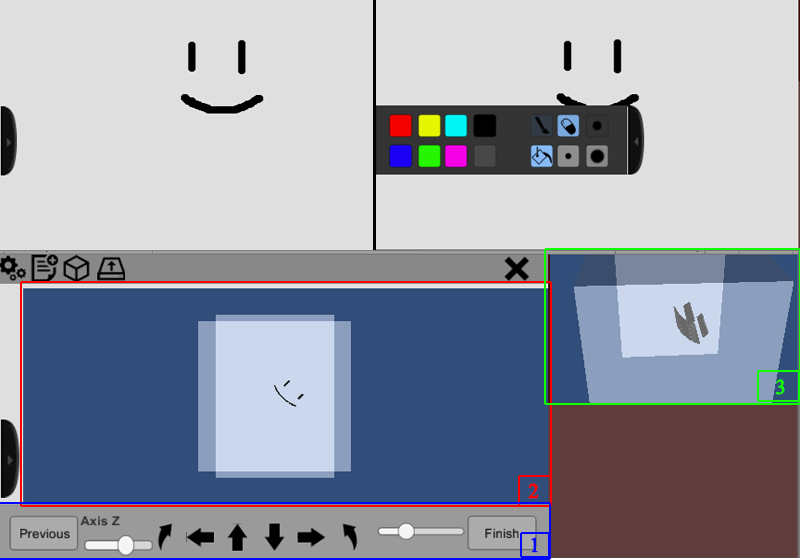
\includegraphics[scale=0.5]{images/Cmt_placer.png}}
		
		Une fois le dessin extrudé, pour le placer dans l'environnement 3D, l'utilisateur pourra à l'aide d'un menu (1) orienté et redimensionné la figure selon chacun de ses axes les un après les autres. Pour se retrouver dans l'environnement, il aura une caméra qui suit l'objet selon l'axe courant (2). Et une caméra amovible et zoomable qui filmera l'ensemble de la scène déjà créée (3). Ici les cubes sont des objets créés précédemment qui sont passés en transparent pour faciliter la lisibilité.\newline\newline

		Une fois tout ces points définis , nous avons pu passer à l'étape suivante, c'est-à-dire l'architecture du logiciel.
		
	\section{Architecture logicielle}
	
				\centerline{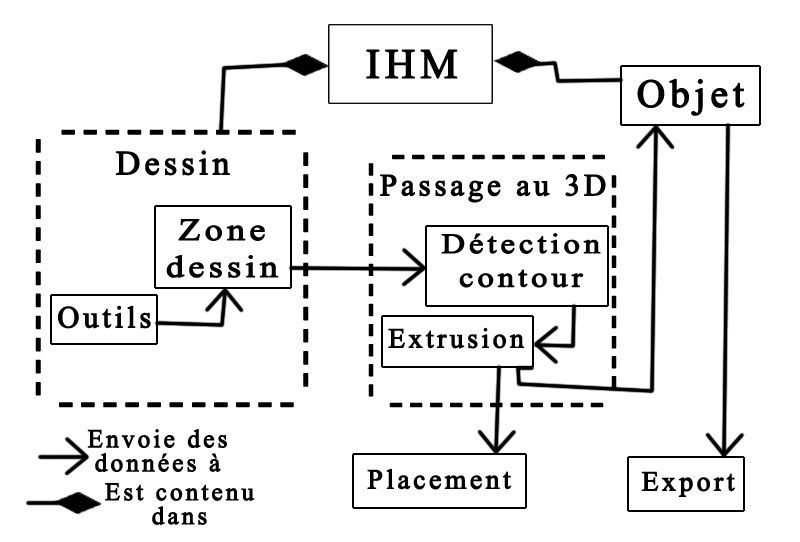
\includegraphics[scale=0.5]{images/archi.png}}
	
		%découpage des tâches et répartition du travail + explication séances hebdomadaires
		Dès le début du projet, nous nous sommes divisés le travail et nous avons hébergé notre projet sous GitHub afin que chacun puisse avancer sans pour autant devoir attendre le travail d'un autre membre de notre équipe. Nous avons repéré les axes centraux du développement qui sont : l'affichage de la fenêtre de l'application, la capture et l'affichage du dessin fait par l'utilisateur, l'extrusion de la forme dessinée, le placement de celle-ci, et enfin l'exportation de la figure finale sur un serveur Unity. Ceux-ci ont donc été partagés entre nous.
		
		Afin de faire un point régulier et d'être sûr de répondre aux exigences de notre encadrant, nous nous sommes réunis hebdomadairement. Au cours de ces séances, nous pouvions ainsi voir le travail effectué par les différents membres de notre projet et nous pouvions bénéficier de l'expérience de M. François LEHERICEY avec Unity pour les problèmes dont nous ne trouvions pas les solutions.

	\section{Présentation de l'application}
		%combien de temps passé pour chaque tâche
		%Problèmes rencontrées et solutions apportées, en quoi ces solutions ont été utilisées par la suite
		\subsection{L'IHM}
			Nous devions d'abord créer le design de l'Interface Homme-Machine (IHM). Nous avons défini sur papier à quoi devaient ressembler les divers menus. Afin de les mettre en place sous Unity, nous avons dû nous servir de la mise à jour 4.6 qui contient un système de fenêtres adapté à la création de menus (UI), sortie fin novembre 2014. Au vu de sa date de sortie récente, nous avions accès à peu d'aides sur Internet. Après une avancée assez laborieuse sur le début, nous avons réussi à mettre en place le canevas\footnote{Un canvas, dans Unity, est une zone où l'on peut insérer et positionner d'autres objets.} principal. 
			
			Le temps passé sur cette partie, nous avons permis d'acquérir les connaissances nécessaires sur les outils UI d'Unity et donc d'avancer plus rapidement dans la suite du développement. De plus, les différents boutons étaient en place et n'attendaient plus que les scripts écrits dans les autres parties.
		
		\subsection{Le dessin}
			La capture du dessin étant une partie lourde, nous avons décidé de séparer les outils de cette partie. C'est la personne en charge de l'IHM, donc déjà accoutumée avec les menus qui s'en sont occupés.
		
		
			\subsubsection{Les outils}				
				Suite directe de l'IHM, un sous-menu coulissant devait être présent pour pouvoir choisir les outils de dessin. Pour rendre le menu coulissant, la solution qui nous a paru la plus adaptée est de se servir de la gestion des animations d'Unity. Une fois celles-ci faites, elles ont été liées à des boutons pour les enclencher.
					
				Dans cette partie la difficulté était de choisir comment coder la sélection d'outils. Pour cela, nous avons choisi de créer une énumération pour chaque ensemble d'outils (couleurs, diamètres, pinceau/gomme/pot de peinture). Des fonctions pour récupérer les outils courants ont été implantées, pour permettre au reste de l'application d'avoir connaissance de l'état des outils. De même des fonctions de Set\footnote{Une fonction de Set est un mutateur. Les mutateurs permettent de changer l'état de données membres tout en vérifiant si la valeur que l'on veut donner à la donnée membre respecte les normes de celle-ci ou diverses règles de cohérence.\emph{Wikipedia}} ont été liées aux boutons appropriés. Pour respecter les droits d'images, nous avons dessiné nous-même les icônes.
				
				Cette partie n'était pas très compliquée en elle-même. Après des tests utilisateurs, nous avons accéléré les animations. Et au cours du développement, ces animations ont dû être plusieurs fois refaites, car elles déclenchaient des bugs non expliqués.
			\subsubsection{La zone de dessin}
			
			C'est pour nous la première étape de la création d'un objet 3D. À la suite de cette étape, nous souhaitions obtenir une image à extruder. Les images sont appelées textures sous Unity. Nous avons utilisé un plan comme objet de référence pour la zone de dessin. Nous nous sommes rendus compte plus tard que la texture de base ne prenait pas l'alpha\footnote{C'est à dire la transparence} en compte, or nous souhaitions disposer d'une image où seul les parties coloriées seraient extrudées. Nous avons donc précisé, lors de la création de la texture, vouloir un type RGB32, pour avoir un fond transparent.
			
			Un premier problème apparut alors quant au dimensionnement de cette zone de dessin. Le plan ayant une taille précise, il fallait être capable de modifier sa taille par rapport à celle du canevas. Nous avons donc rédigé un script qui initialise la dimension de la zone de dessin, autant pour le plan que pour la texture qui lui est associée.
			
			Il fallait ensuite être capable de dessiner sur la texture, or l'objet (le plan ici) et la texture ont des dimensions différentes : nous avons d'abord tenté de modifier la texture à l'endroit où l'on cliquait, mais il y avait toujours un décalage à l'affichage. Finalement, la solution la plus efficace fut de projeter un Ray, objet monodirectionnel qui traverse l'espace, au moment où l'on clique dans la zone de dessin, et de trouver le pixel à l'intersection de ces deux objets. On a ainsi pu, dans un premier temps, modifier un pixel en cliquant dessus. Ensuite, pour garder un tracé continu, nous avons implémenté une méthode qui trace la droite entre le dernier point colorié, et le point sur lequel on clique. Il restait à faire le lien entre la zone de dessin, et les différents outils définis plus tôt. Ainsi, la zone de dessin va chercher les différentes couleurs, la largeur du trait, et les outils à utiliser dans le menu déroulant. Nous avons aussi implémenté des méthodes "eraser" et "bucket", capables de gommer et remplir rapidement une surface.
			
		\hypertarget{ancre}{
		\subsection{L'extrusion}}
		\label{extrusion}
		L'extrusion est une autre tâche importante du projet. En effet, il faut à partir d'une texture, créer un objet en 3D. Pour ce faire, nous sommes partis d'une extension Unity déjà existante : UCLA Mesh Creator. C'est un créateur d'objets 3D, à partir d'une texture. Seulement, il a fallu reprendre le code pour l'adapter à notre utilisation. Initialement, cette application sert à créer rapidement et simplement un objet afin de pouvoir l'insérer dans son jeu. De plus, il est possible de la faire fonctionner uniquement en mode "édition". Il y a deux modes quand on l'on travaille sous Unity : le mode "édition", qui nous permet de créer des scènes avec nos objets, nos animations, et un mode "jeu" où l'on voit le rendu final avec lequel l'utilisateur interagira. Nous nous sommes donc concentrés sur l'adaptation du code déjà existant plutôt que sur la recherche et l'implémentation d'un ou plusieurs algorithmes afin de détecter les contours d'une image. Seulement, comme c'est une adaptation, il y a eu une longue phase de compréhension et de test afin de faire fonctionner comme il faut cette application. 
		\subsection{Placement de la figure}
		
			Pour placer une figure dans le décor 3D, il faut créer des menus pour diriger celle-ci. Et intégrer une caméra qui filmerait l'objet courant selon ses axes. Après de multiples recherches sur la gestion des caméras Unity, nous avons finalement réussi à écrire un script assurant ce suivi avec une possibilité de changer aisément l'axe de vue. Ensuite il y a eu la mise en place d'un menu pour diriger notre figure. Celui-ci est relativement simple à mettre en place aux vues de ce que l'on a réalisé précédemment dans l'IHM. La difficulté de cette partie est de concevoir un script pour modifier la taille de notre figure.

		\subsection{La gestion de la liste des figures}
		\subsection{L'envoi}
			Un fois l'objet en 3D créé, nous devons l'envoyer à un serveur qui affichera cet objet dans une scène 3D.
			Nous avons tout d'abord pensé utiliser les assets , c'est-à-dire les classes, propres à Unity gérant le réseau entre différentes applications Unity. Mais nous avons très vite été confronté à un problème: Unity est avant tout un moteur de jeu, et les classes sont développées dans cette optique.
			Par exemple, si on examine un jeu en multijoueur, on se rend compte que le contenu, les objets, sont déjà tous connus du serveur et des clients. Or, nous créons un objet à partir de zéro, et nous voulons l'envoyer au serveur. On ne peut donc pas utiliser les classes dédiées au réseau. Nous avons donc décidé de nous orienter vers d'autres solutions.
			Comme notre application a été codée en C\#, nous avons décidé de passer par les classes de .NET pour la gestion du réseau.
			La nouvelle piste a été d'utiliser les "sockets" ou connecteurs réseau qui permettent, entre autre, de connecter un serveur et un client et d'échanger des données. Nous avons dû choisir parmi deux protocoles d'échange de données: UDP et TCP.
			M. François LEHERICEY nous a informé que le protocole UDP ne fonctionnerait pas sur le réseau de l'IRISA, ainsi nous avons choisi le protocole TCP.
	\section{Organisation du travail}
	\section{Objectifs}
		%Qu'est-ce qu'on a : changé, abandonné ...
		Au cours de l'avancement du projet, nous avons du faire certains choix, et changer ou abandonner certaines de nos idées initiales.
		Pour le dessin, nous nous sommes contenté de trois tailles pour l'outil de coloriage.
		La possibilité de sauvegarder des objets n'était pas, à l'origine, une des fonctionnalités de l'application. Mais en se concertant, nous nous sommes rendu compte qu'une personne aimerait sûrement pouvoir réutiliser ses objets dans la construction d'autres objets. Si toutes les autres fonctionnalités de l'application sont opérationnelles, la sauvegarde serait un objectif potentiel à rajouter.
		Globalement, nous sommes arrivés à un résultat très proche de notre conception initiale de l'application.
	\section{Conclusion}
		%Ce que l'on se souviendra du projet
		%Si c'était à refaire, quoi changer?
		%Quelles sont les évolutions que l'on pourrait apporter à notre application finale
			Nous en retenons qu'Unity est un outil puissant, mais pas encore adapté à la création de menus, et orienté pair-à-pair. Ce travail fut aussi une bonne initiation à la gestion de projet, avec l'utilisation de Git. Il en ressort aussi qu'il est crucial de se donner des tâches précises et des délais à respecter pour arriver au bout d'un projet dans les temps impartis. Cela évite qu'une partie minime du projet ne nous accapare tout notre temps.
			
			Si l'on nous présentait ce projet à nouveau, nous changerions notre méthode de travail sur plusieurs points. Notamment, nous passerions moins de temps sur l'état de l'art; il était presque sûr qu'Unity serait notre choix comme outil de développement. Ensuite, nous procéderions à un partage des recherches et des réflexions aux premiers instants du projet. Nous commencerions à apprendre à utiliser Unity dès le mois d'Octobre, car ce manque de connaissances nous a relenti par la suite. Nous étions parfois bloqués par des détails, ou nous trouvions des solutions sans les comprendre entièrement, menant à d'autres problèmes par la suite. Mais le manque de temps ne nous permettait pas de faire autrement.
			
			Notre application a encore plusieurs voies d'améliorations possibles. Comme l'implantation d'outils pour faire des sphères, avec des extrusions circulaires.
	
	\section{Remerciements}
		Nous souhaitons tout d'abord remercier Monsieur François LEHERICEY pour sa disponibilité ainsi que pour ses précieuses informations.
		
		Nous voudrions également remercier Monsieur Bertrand COUASNON pour son apport de connaissances ainsi que son aide dans l'élaboration de nos différentes présentations.
	
\end{document}